\definecolor{aohomo}{HTML}{0072B2}
\definecolor{aolumo}{HTML}{D55E00}

% The data are read from the same CP2K outputs as
% Fig.~\ref{fig:ao-frontier-results}. For GW100, HOMO and LUMO values are
% mean absolute errors against the 99 aug-TZVP reference calculations.

% Panel (a): GW100, PBE frontier-orbital MAEs.
\def\aoleftinitiala{(0.55,0.205585) (1.95,0.134159) (3.45,0.034767) (4.85,0.028779)}
\def\aoleftoptimizeda{(0.55,0.232306) (1.95,0.127625) (3.45,0.038852) (4.85,0.029932)}
\def\aorightinitiala{(0.55,0.301529) (1.95,0.228267) (3.45,0.110943) (4.85,0.104606)}
\def\aorightoptimizeda{(0.55,0.411909) (1.95,0.176333) (3.45,0.073679) (4.85,0.055333)}
\def\aoleftlabela{HOMO MAE (eV)}
\def\aorightlabela{LUMO MAE (eV)}
\def\aopaneltitlea{\textit{GW}100, PBE}
\def\aoleftymina{0}
\def\aoleftymaxa{0.50}
\def\aoleftyticksa{{0,0.1,0.2,0.3,0.4,0.5}}
\def\aoleftminorticksa{{-1}}
\def\aorightymina{0}
\def\aorightymaxa{0.50}
\def\aorightyticksa{{0,0.1,0.2,0.3,0.4,0.5}}
\def\aorightminorticksa{{-1}}
\def\aoxticklabelsa{{},{},{},{}}

% Panel (b): GW100, G0W0 frontier-orbital MAEs.
\def\aoleftinitialb{(0.55,0.803740) (1.95,0.495191) (3.45,0.242391) (4.85,0.188357)}
\def\aoleftoptimizedb{(0.55,0.765005) (1.95,0.646524) (3.45,0.298415) (4.85,0.221548)}
\def\aorightinitialb{(0.55,1.259532) (1.95,0.664340) (3.45,0.402577) (4.85,0.339589)}
\def\aorightoptimizedb{(0.55,1.506462) (1.95,0.676458) (3.45,0.339492) (4.85,0.260025)}
\def\aoleftlabelb{HOMO MAE (eV)}
\def\aorightlabelb{LUMO MAE (eV)}
\def\aopaneltitleb{\textit{GW}100, $G_0W_0$}
\def\aoleftyminb{0}
\def\aoleftymaxb{1.6}
\def\aoleftyticksb{{0,0.4,0.8,1.2,1.6}}
\def\aoleftminorticksb{{0.1,0.2,0.3,0.5,0.6,0.7,0.9,1.0,1.1,1.3,1.4,1.5}}
\def\aorightyminb{0}
\def\aorightymaxb{1.6}
\def\aorightyticksb{{0,0.4,0.8,1.2,1.6}}
\def\aorightminorticksb{{0.1,0.2,0.3,0.5,0.6,0.7,0.9,1.0,1.1,1.3,1.4,1.5}}
\def\aoxticklabelsb{{},{},{},{}}

% Panel (c): Si45H56, PBE frontier-orbital energies.
\def\aoleftinitialc{(0.55,-5.925) (1.95,-5.861) (3.45,-5.876) (4.85,-5.874)}
\def\aoleftoptimizedc{(0.55,-5.944) (1.95,-5.883) (3.45,-5.857) (4.85,-5.859)}
\def\aorightinitialc{(0.55,-2.280) (1.95,-2.539) (3.45,-2.702) (4.85,-2.710)}
\def\aorightoptimizedc{(0.55,-2.390) (1.95,-2.719) (3.45,-2.702) (4.85,-2.711)}
\def\aoleftlabelc{HOMO (eV)}
\def\aorightlabelc{LUMO (eV)}
\def\aopaneltitlec{Si$_{45}$H$_{56}$, PBE}
\def\aoleftyminc{-6.3}
\def\aoleftymaxc{-5.5}
\def\aoleftyticksc{{-6.2,-6.0,-5.8,-5.6}}
\def\aoleftminorticksc{{-6.1,-5.9,-5.7}}
\def\aorightyminc{-2.9}
\def\aorightymaxc{-2.1}
\def\aorightyticksc{{-2.8,-2.6,-2.4,-2.2}}
\def\aorightminorticksc{{-2.7,-2.5,-2.3}}
\def\aoxticklabelsc{{},{},{},{}}

% Panel (d): Si45H56, G0W0 frontier-orbital energies.
\def\aoleftinitiald{(0.55,-6.565) (1.95,-6.872) (3.45,-7.092) (4.85,-7.193)}
\def\aoleftoptimizedd{(0.55,-6.602) (1.95,-6.919) (3.45,-7.065) (4.85,-7.198)}
\def\aorightinitiald{(0.55,-0.264) (1.95,-0.982) (3.45,-1.344) (4.85,-1.500)}
\def\aorightoptimizedd{(0.55,-0.397) (1.95,-1.093) (3.45,-1.322) (4.85,-1.495)}
\def\aoleftlabeld{HOMO (eV)}
\def\aorightlabeld{LUMO (eV)}
\def\aopaneltitled{Si$_{45}$H$_{56}$, $G_0W_0$}
\def\aoleftymind{-7.6}
\def\aoleftymaxd{-6.0}
\def\aoleftyticksd{{-7.4,-7.0,-6.6,-6.2}}
\def\aoleftminorticksd{{-7.5,-7.3,-7.2,-7.1,-6.9,-6.8,-6.7,-6.5,-6.4,-6.3,-6.1}}
\def\aorightymind{-1.6}
\def\aorightymaxd{0.0}
\def\aorightyticksd{{-1.4,-1.0,-0.6,-0.2}}
\def\aorightminorticksd{{-1.5,-1.3,-1.2,-1.1,-0.9,-0.8,-0.7,-0.5,-0.4,-0.3,-0.1}}
\def\aoxticklabelsd{{},{},{},{}}

\newcommand{\aodualpanel}[5]{%
  \begin{axis}[
    name=ao#1left,
    at={(#2,#3)},anchor=south west,
    width=5.80cm,height=3.8cm,scale only axis,
    xmin=0.35,xmax=5.05,
    xtick={0.55,1.95,3.45,4.85},
    xticklabels=\empty,
    ymin=\csname aoleftymin#1\endcsname,
    ymax=\csname aoleftymax#1\endcsname,
    ytick=\csname aoleftyticks#1\endcsname,
    minor ytick=\csname aoleftminorticks#1\endcsname,
    ylabel={\csname aoleftlabel#1\endcsname},
    axis y line*=left,axis x line*=bottom,
    x axis line style={black,line width=0.65pt},
    y axis line style={aohomo,line width=0.65pt},
    y tick label style={font=\normalsize,text=aohomo,
      /pgf/number format/fixed,/pgf/number format/precision=1,
      /pgf/number format/fixed zerofill},
    y label style={font=\normalsize,text=aohomo},
    grid=both,
    major grid style={draw=gray!35,line width=0.35pt},
    minor grid style={draw=gray!18,line width=0.25pt},
    tick align=outside,major tick length=2pt,minor tick length=1pt,
    tick label style={font=\normalsize},
    every axis plot/.append style={line width=1.05pt,mark size=2.0pt},
    clip=false,
  ]
    \addplot[color=aohomo,dashed,mark=triangle*,
      mark options={solid,fill=aohomo,draw=aohomo}]
      coordinates {\csname aoleftinitial#1\endcsname};
    \addplot[color=aohomo,solid,mark=*,
      mark options={solid,fill=aohomo,draw=aohomo}]
      coordinates {\csname aoleftoptimized#1\endcsname};
    \node[anchor=north west,fill=white,fill opacity=1,text opacity=1,
      inner sep=1.5pt,font=\normalsize]
      at (rel axis cs:#5,0.985) {(#1)};
    \node[anchor=north,draw=gray!45,rounded corners=1pt,
      fill=white,fill opacity=0.94,text opacity=1,inner sep=2pt,
      font=\normalsize,align=center]
      at (rel axis cs:0.50,0.985) {\csname aopaneltitle#1\endcsname};
    \draw[black,line width=0.65pt]
      (rel axis cs:0,0) -- (rel axis cs:1,0);
    \draw[black,line width=0.65pt]
      (rel axis cs:0,1) -- (rel axis cs:1,1);
    \ifnum#4=1
      \node[anchor=north,font=\small,xshift=-2.0mm,yshift=-1.0mm]
        at (rel axis cs:0.043,0) {aug-SZV-t1};
      \node[anchor=north,font=\small,xshift=-0.5mm,yshift=-1.0mm]
        at (rel axis cs:0.340,0) {aug-SZV-t2};
      \node[anchor=north,font=\small,xshift=0.5mm,yshift=-1.0mm]
        at (rel axis cs:0.660,0) {aug-DZVP-t1};
      \node[anchor=north,font=\small,xshift=4.0mm,yshift=-1.0mm]
        at (rel axis cs:0.957,0) {aug-DZVP-t2};
    \fi
  \end{axis}
  \begin{axis}[
    at={(ao#1left.south west)},anchor=south west,
    width=5.80cm,height=3.8cm,scale only axis,
    xmin=0.35,xmax=5.05,xtick=\empty,
    ymin=\csname aorightymin#1\endcsname,
    ymax=\csname aorightymax#1\endcsname,
    ytick=\csname aorightyticks#1\endcsname,
    minor ytick=\csname aorightminorticks#1\endcsname,
    ylabel={\csname aorightlabel#1\endcsname},
    axis y line*=right,axis x line=none,
    y axis line style={aolumo,line width=0.65pt},
    y tick label style={font=\normalsize,text=aolumo,
      /pgf/number format/fixed,/pgf/number format/precision=1,
      /pgf/number format/fixed zerofill},
    y label style={font=\normalsize,text=aolumo},
    tick align=outside,major tick length=2pt,minor tick length=1pt,
    every axis plot/.append style={line width=1.05pt,mark size=2.0pt},
  ]
    \addplot[color=aolumo,dashed,mark=triangle*,
      mark options={solid,fill=aolumo,draw=aolumo}]
      coordinates {\csname aorightinitial#1\endcsname};
    \addplot[color=aolumo,solid,mark=*,
      mark options={solid,fill=aolumo,draw=aolumo}]
      coordinates {\csname aorightoptimized#1\endcsname};
  \end{axis}
}

\begin{figure*}[t!]
  \centering
  \makebox[\textwidth][c]{%
  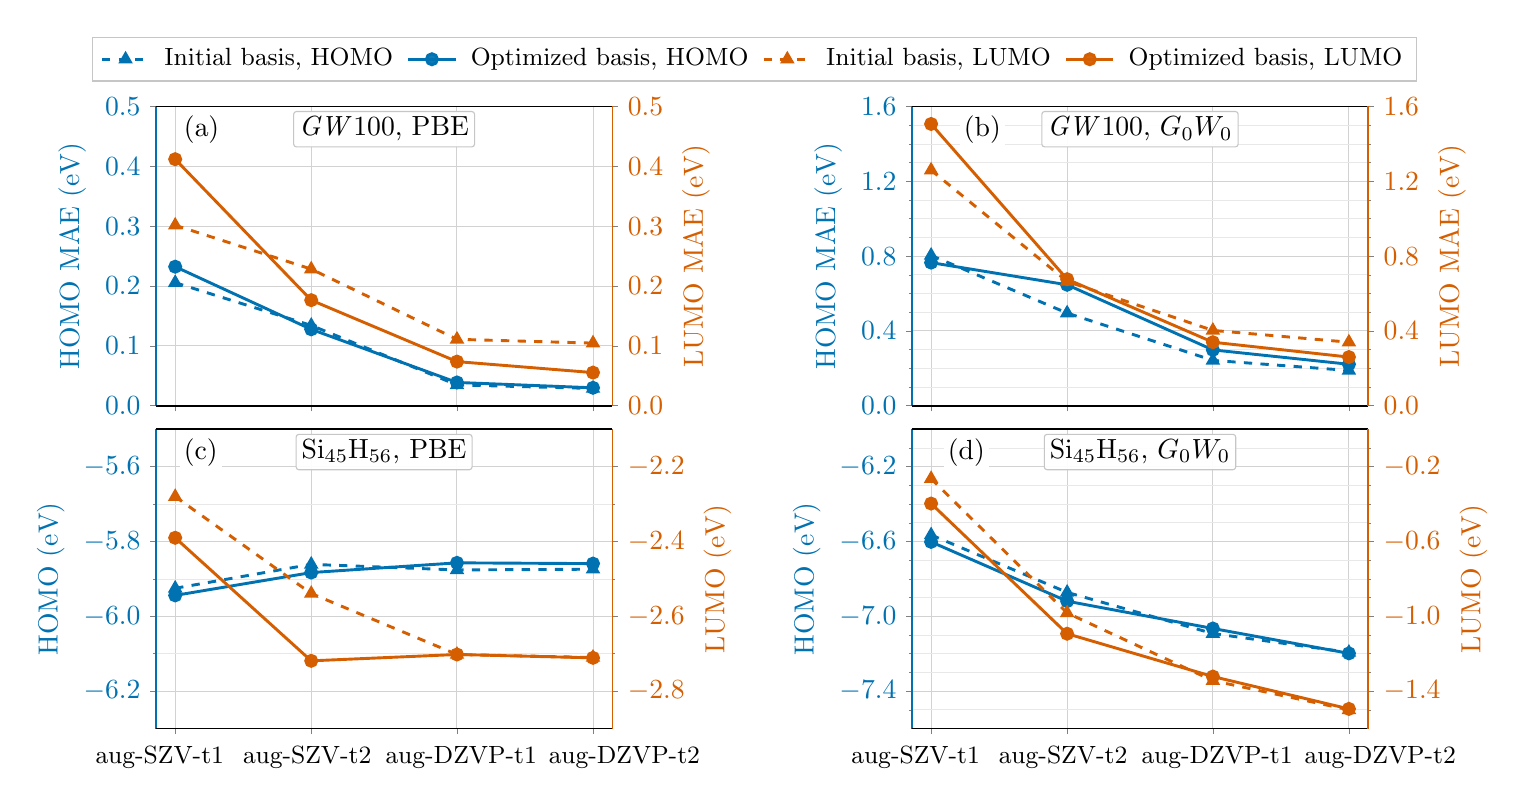
\begin{tikzpicture}
    \begin{axis}[
      hide axis,width=0pt,height=0pt,scale only axis,
      legend to name=ao-frontier-orbital-legend,
      legend columns=4,
      legend style={font=\small,draw=gray!45,fill=white,
        fill opacity=0.94,text opacity=1,cells={anchor=west},
        row sep=0pt,column sep=3pt},
    ]
      \addplot[draw=none,mark=none,forget plot] coordinates {(0,0)};
      \addlegendimage{color=aohomo,dashed,line width=1.05pt,mark=triangle*,
        mark options={solid,fill=aohomo,draw=aohomo},mark size=2.0pt}
      \addlegendentry{Initial basis, HOMO}
      \addlegendimage{color=aohomo,solid,line width=1.05pt,mark=*,
        mark options={solid,fill=aohomo,draw=aohomo},mark size=2.0pt}
      \addlegendentry{Optimized basis, HOMO}
      \addlegendimage{color=aolumo,dashed,line width=1.05pt,mark=triangle*,
        mark options={solid,fill=aolumo,draw=aolumo},mark size=2.0pt}
      \addlegendentry{Initial basis, LUMO}
      \addlegendimage{color=aolumo,solid,line width=1.05pt,mark=*,
        mark options={solid,fill=aolumo,draw=aolumo},mark size=2.0pt}
      \addlegendentry{Optimized basis, LUMO}
    \end{axis}
    \node at (7.60cm,8.50cm) {\pgfplotslegendfromname{ao-frontier-orbital-legend}};

    \aodualpanel{a}{0cm}{4.1cm}{0}{0.051}
    \aodualpanel{b}{9.60cm}{4.1cm}{0}{0.104}
    \aodualpanel{c}{0cm}{0cm}{1}{0.051}
    \aodualpanel{d}{9.60cm}{0cm}{1}{0.069}
  \end{tikzpicture}%
  }
  \par\vspace{-0.2cm}
  \caption{PBE and $G_0W_0$ HOMO and LUMO energies for the initial and
  optimized augmented MOLOPT basis sets. The underlying calculations are the
  same as in Figure~\ref{fig:ao-frontier-results}.}
  \label{fig:ao-frontier-orbital-energies}
  \vspace{-0.8cm}
\end{figure*}
